\documentclass[arhiv]{izpit}
\usepackage{fouriernc}
\usepackage{tikz}
\usepackage{censor}
\usepackage{paralist}

\begin{document}

\izpit{Programiranje I: 1.\ izpit}{3.\ svečan 2014}{
  Čas reševanja je 150 minut.
  Doseženih 100 točk šteje za maksimalno oceno.
  Veliko uspeha!
}

%%%%%%%%%%%%%%%%%%%%%%%%%%%%%%%%%%%%%%%%%%%%%%%%%%%%%%%%%%%%%%%%%%%%%%
\naloga[Mafija, 10 + 10 + 10 točk]
V neki mafijski organizaciji so člani urejeni hierarhično. Vsakdo razen botra (vrhovnega šefa) ima natanko enega
nadrejenega. Vsak mafijec ima lahko pod seboj največ dva podrejena (levega in desnega). Primer takšne mafijske
organizacije:
$$
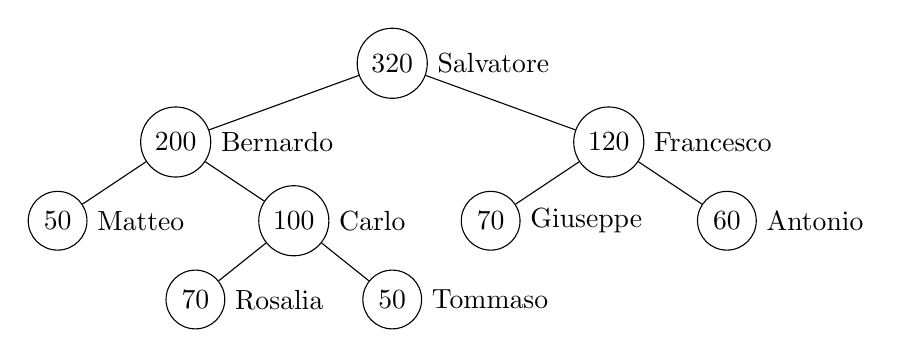
\begin{tikzpicture}[level distance=1cm,
    level 1/.style={sibling distance=5.5cm},
    level 2/.style={sibling distance=3cm},
    level 3/.style={sibling distance=2.5cm}
    ]
    \node[circle, draw, label=0:Salvatore] (d) {320}
      child {node[circle, draw, label=0:Bernardo] {200}
        child {node[circle, draw, label=0:Matteo] {50}}
        child {node[circle, draw, label=0:Carlo] {100}
          child {node[circle, draw, label=0:Rosalia] {70}}
          child {node[circle, draw, label=0:Tommaso] {50}}
        }
      }
      child {node[circle, draw, label=0:Francesco] {120}
        child {node[circle, draw, label=0:Giuseppe] {70}}
        child {node[circle, draw, label=0:Antonio] {60}}
      };
  \end{tikzpicture}
$$
Mafijci morajo zbirati denar s kriminalnimi dejavnostmi. Tisti, ki imajo podrejene, pa ga poleg tega poberejo
še od svojih podrejenih. Ves ``prisluženi'' in prejeti denar morajo oddati svojemu nadrejenemu.

Boter je posumil, da nekateri člani goljufajo. Nekaj denarja, ki ga poberejo od podrejenih, zadržijo zase. Od vsakega
člana je pridobil podatek o tem, koliko denarja je oddal naprej. Podatke je shranil v podatkovno strukturo \texttt{Drevo}, ki je že implementirana.

\podnaloga[10 točk]
Botra zanima, koliko denarja zaradi goljufov ``ponikne''. Želi, da sestavite funkcijo \texttt{naloga1a(self)}, ki vrne skupno vsoto denarja, ki ponikne. Primer (če \texttt{d} ustreza zgornji sliki):
%
\begin{verbatim}
>>> d.naloga1a()
30
\end{verbatim}

\podnaloga[10 točk]
Ko je boter dognal, koliko denarja ponikne, je totalno po\censor{pizdil}. Pri priči hoče imeti imena vseh goljufov!
Napišite funkcijo \texttt{naloga1b(self)}, ki vrne množico goljufov. Vsak goljuf naj bo predstavljen z naborom. Prva kompotenta naj bo ime goljufa, druga komponenta pa količina denarja, ki ga je utajil. Primer:
%
\begin{verbatim}
>>> d.naloga1b()
{('Carlo', 20), ('Francesco', 10)}
\end{verbatim}

\podnaloga[10 točk]
Botru se dozdeva, da so najbolj pridne \emph{majhne ribe}. To so tisti mafijci, ki nimajo pod seboj nobenega podrejenega. Tistim, ki imajo podrejene, se reče \emph{velike ribe}. Napišite funkcijo \texttt{naloga1c(self)}, ki vrne par (nabor) dveh števili, pri čemer je:
\begin{compactitem}
\item 1.\ število skupna vsota denarja, ki ga zaslužijo majhne ribe;
\item 2.\ število skupna vsota denarja, ki ga zaslužijo velike ribe (brez pobirkov od podrejenih). 
\end{compactitem}
Primer:
%
\begin{verbatim}
>>> d.naloga1c()
(300, 50)
\end{verbatim}

%%%%%%%%%%%%%%%%%%%%%%%%%%%%%%%%%%%%%%%%%%%%%%%%%%%%%%%%%%%%%%%%%%%%%%
\naloga[Poravnava besedila, 20 + 15 točk]

\emph{Besedilo} je zaporedje znakov, ki so zapisani v neki datoteki. \emph{Prazni znaki} so: presledek, tabulator in skok v novo vrstico (\verb+' '+, \verb+'\t'+ in \verb+'\n'+). \emph{Beseda} pa bo za nas maksimalni strnjeni podniz, ki ne vsebuje praznih znakov. V besedilu
\begin{verbatim*}
Na to se cesar začudi in pravi: "Ako so brusi, pokaj so pa v vrečah?" 
\end{verbatim*}
podniz \verb+"Ako+ po naši definiciji je beseda, \verb+Ako+ pa ne (saj ni maksimalen).

\podnaloga[20 točk]
Sestavite funkcijo \texttt{naloga2a(vhodna, izhodna, w)}, ki besedilo iz datoteke z imenom \texttt{vhodna}
prepiše na datoteko z imenom \texttt{izhodna}, pri tem pa naj odstrani odvečne prazne znake. Velja naj naslednje:
\begin{compactitem}
\item vsaka vrstica naj bo kar se da dolga;
\item nobena vrstica naj ne vsebuje več kot \texttt{w} znakov (pri čemer znaka \verb+'\n'+ na koncu vrstice ne
štejemo);
\item besede znotraj
iste vrstice naj bodo ločene s po enim presledkom (ne glede na to s katerimi in koliko praznimi znaki so
ločene v originalnem besedilu).
\end{compactitem}
Predpostavite, da dolžina nobene besede ni več kot \texttt{w}.

Primer: Če je na datoteki \texttt{krpan.txt} besedilo
%
\begin{verbatim*}
"I kaj
pa nosiš v
  tovoru?" cesar dalje vpraša.

Krpan se naglo izmisli in reče: "I kaj? Kresilno gobo pa nekaj brusov
sem naložil, gospod!"
\end{verbatim*}
%
naj bo po klicu funkcije
%
\begin{verbatim}
>>> naloga2a('krpan.txt', 'lepo.txt', 30)
\end{verbatim}
%
v datoteki \texttt{lepo.txt} besedilo
%
\begin{verbatim*}
"I kaj pa nosiš v tovoru?"
cesar dalje vpraša. Krpan se
naglo izmisli in reče: "I kaj?
Kresilno gobo pa nekaj brusov
sem naložil, gospod!"
\end{verbatim*}
%
\podnaloga[15 točk] Sestavite funkcijo \texttt{naloga2b(vhodna, izhodna, w)}, ki besedilo oblikuje tako, da bo še
obojestransko poravnano. Obojestransko poravnavo dosežemo s tem, da med besede znotraj vrstice postavimo več presledkov. Presledki
naj bodo razporejeni tako, da je razlika med dolžino največje in najmanjše luknje\footnote{Za tiste, ki niste uganili:
\emph{luknja} pomeni maksimalno strnjeno zaporedje enega ali več presledkov.} znotraj iste vrstice kvečjemu 1,
ta večje luknje pa naj bodo vse na desni strani vrstice.

Primer: Po klicu funkcije
%
\begin{verbatim}
>>> naloga2b('krpan.txt', 'obojestransko.txt', 30)
\end{verbatim}
%
naj bo v datoteki \texttt{obojestransko.txt} besedilo
%
\begin{verbatim*}
"I kaj  pa  nosiš  v  tovoru?"
cesar dalje vpraša.  Krpan  se
naglo izmisli in reče: "I kaj?
Kresilno gobo pa nekaj  brusov
sem     naložil,      gospod!"
\end{verbatim*}

%%%%%%%%%%%%%%%%%%%%%%%%%%%%%%%%%%%%%%%%%%%%%%%%%%%%%%%%%%%%%%%%%%%%%%
\naloga[Izštevanka, 25 točk]

\begin{verse}
Cinca Binca, v luknji miš,\\
če jo ujameš, ne loviš.\\
Kdor pa miške ne ulovi,\\
ta za kazen naj miži.\\
En, dva, tri,\\
en, dva, tri,\\
zdaj mižiš -- ti!
\end{verse}

V \emph{Mathematici} sestavite funkcijo \texttt{naloga3[l\_, k\_]}, ki ``simulira'' izštevanko. Predstavljajmo si, da je seznam \texttt{l} cikličen (udeleženci stojijo v krogu). Šteti začnemo pri prvem elementu in preštejemo do \texttt{k}. Tistega, pri katerem smo se ustavili, izločimo. Nato ponovno štejemo do \texttt{k}. S štetjem začnemo pri tistem elementu, ki je desno od pravkar izločenega. Elementov, ki smo jih že izločili, pri štetju ne upoštevamo več. Izštevanko se gremo toliko časa, dokler ne izločimo vseh elementov. Funkcija naj vrne seznam elementov v takem vrstnem redu, kot smo jih izločali pri izštevanki. Primer:
%
\begin{verbatim}
In[1]:= naloga3[{"Jani", "Tone", "Cilka", "Boris", "Franci", "Ana", "Pero"}, 5]
Out[1]= {"Franci", "Cilka", "Tone", "Boris", "Pero", "Jani", "Ana"}

In[2]:= naloga3[{"Jaka", "Tomaž", "Barbara", "Gašper", "Petra"}, 1337]
Out[2]= {"Tomaž", "Barbara", "Petra", "Jaka", "Gašper"}
\end{verbatim}

%%%%%%%%%%%%%%%%%%%%%%%%%%%%%%%%%%%%%%%%%%%%%%%%%%%%%%%%%%%%%%%%%%%%%%
\naloga[Naključni grafi, 30 točk]

V \emph{Mathematici} sestavite funkcijo \texttt{naloga4[n\_, p\_]}, ki izriše sliko naključnega grafa z \texttt{n} vozlišči. Naključni graf nastane tako, da za vsak par vozlišč med njima z verjetnostjo \texttt{p} potegnemo povezavo.
Vozlišča naj bodo ekvidistančno razporejena po enotski krožnici.

\begin{center}
\begin{tabular}{c@{\hspace{1.5cm}}c@{\hspace{1.5cm}}c}
  \includegraphics[width=4cm]{graf1.pdf}&
  \includegraphics[width=4cm]{graf2.pdf}&
  \includegraphics[width=4cm]{graf3.pdf}\\
  \texttt{naloga4[5, 0.5]} &
  \texttt{naloga4[10, 0.1]} &
  \texttt{naloga4[6, 1.0]}
\end{tabular}
\end{center}

% naloga3[n_] := Graphics[{
%    Table[Line[{{-k, 0}, {-k + 1, 0}}], {k, 1, n, 2}],
%    Table[Line[{{0, -k}, {0, -k + 1}}], {k, 2, n, 2}],
%    Table[Line[{{-k, 0}, {-k, -k}, {0, -k}}], {k, 1, n}]}]

\end{document}

